\section{Experimental evaluation}
\subsection{Data set and processing}
The data set that was obtained from 20 receipts that were manually annotated with the position of each character in them. In total there are 7045 characters. There are 74 different characters, including digits, uppercase and lowercase letters and punctuation. 

The bounding boxes of the characters were extracted from the images. The resulting patches were normalized to have a size of 30x30 pixels and were converted to grayscale. The small images that resulted after this processing were used as the data set for the character recognition problem.

For the character segmentation problem, positive and negative patches were extracted from the images, each containing 40 columns of pixels. The positive example were obtained by taking the leftmost and rightmost columns of the bounding boxes of characters, together with 19 previous columns and 20 columns that followed. The negative examples were obtained by sampling randomly from the middle of a character and taking 19 columns from before and 20 from after.

For the character recognition problem, the labels corresponding to each character were converted to a vector of 74 dimensions, with each dimension corresponding to one possible character value. The value of the dimension corresponding to the character of a data point was set to 1, while all the others were set to 0. 

For the character segmentation problem, the labels were binary: 1 if a certain data point was were a segmentation should occur, 0 otherwise. 
\begin{figure}
\centering
\begin{subfigure}{.5\textwidth}
  \centering
  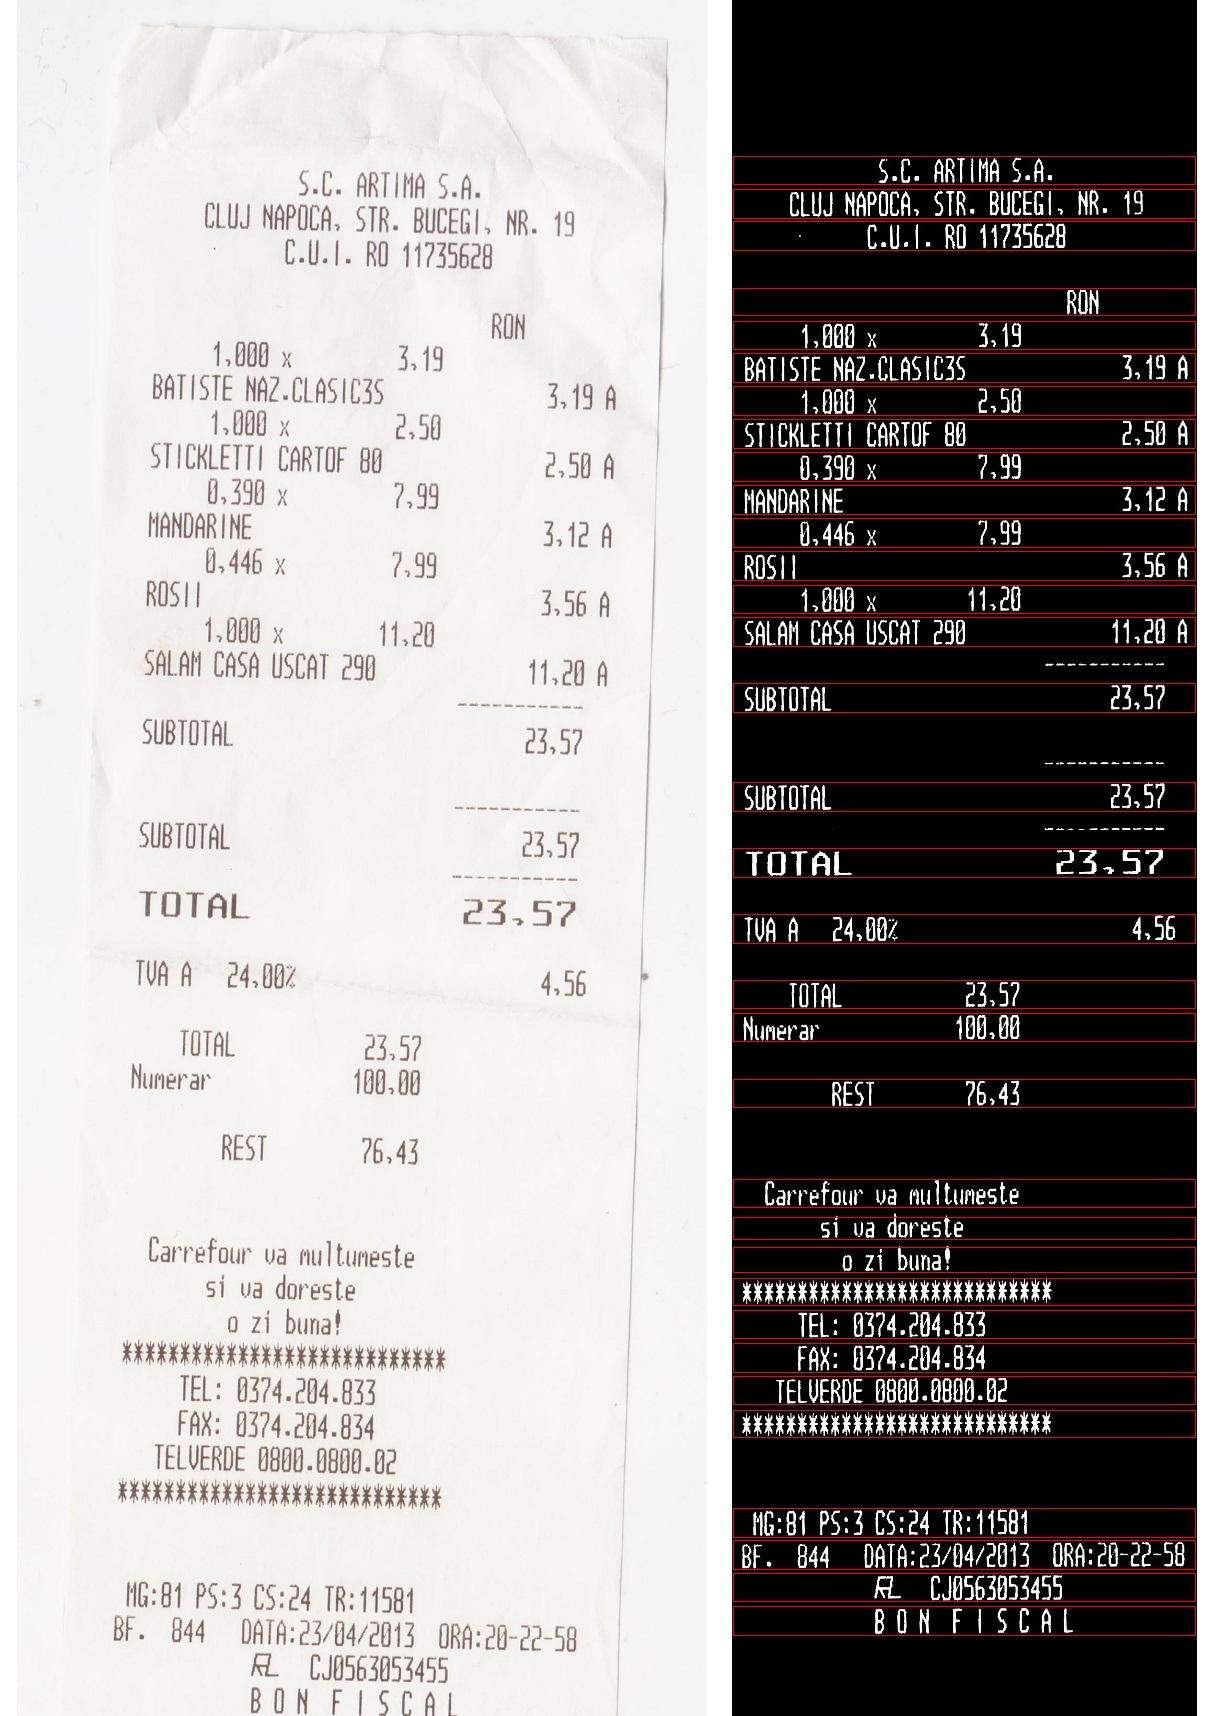
\includegraphics[width=.4\linewidth]{figures/bon1/bon1.jpg}
  \caption{A subfigure}
  \label{fig:sub1}
\end{subfigure}%
\begin{subfigure}{.5\textwidth}
  \centering
  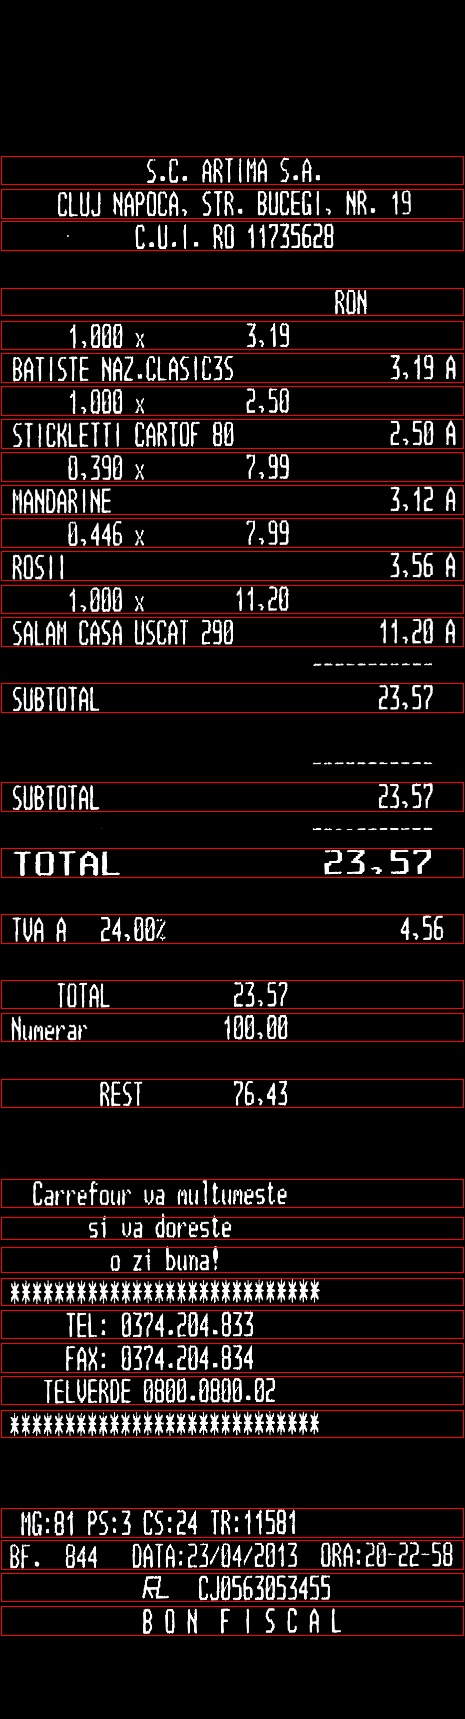
\includegraphics[width=.4\linewidth]{figures/1/1.jpg}
  \caption{A subfigure}
  \label{fig:sub2}
\end{subfigure}
\caption{A figure with two subfigures}
\label{fig:test}
\end{figure}
\subsection{Training and testing}
The data set was shuffled and then split into two parts, one for training and one for testing. The splitting was done in a random way, because the data points are independent and order does not matter. The training set contained 80\% of the data and the test set contained the remaining 20\%. 

All experiments were run multiple types, with the dataset being shuffled each time. In the case of the Random Forests, the multiple runs of the experiments are necessary because the splitting points for the trees and the dataset splits are chosen randomly across runs. 
\subsection{Experiments}

For both tasks, the parameters for the algorithms were selected using cross-validation. In the case of the SVM, the search space was on logarithmic scale from $10^{-2}$ to $10^4$ for the regularization parameter. In the case of the random forest, the number of trees used ranged from 150 to 250, in steps of 50, and the number of features to be sampled at each point varied from using the square root, the base 2 logarithm, 10\% or 30\% of the total number of features. 

Table \ref{table:recog_values} contains the average, maximum and minimum values obtained for the accuracy of the character recognition problem.

% Please add the following required packages to your document preamble:
% \usepackage{booktabs}
\begin{table}[h]
\caption{The errors for the character recognition experiment}
\label{table:recog_values}
\begin{tabular}{llllll}
\hline
Kernel type & Regularization & Min     & Max     & Mean    & Std. dev. \\ \hline
RBF & 0.01 & 0.09141 & 0.09207 & 0.09165 & 0.00030 \\ 
Linear & 0.01 & 0.71585 & 0.71768 & 0.71672 & 0.00075 \\ 
RBF & 1 & 0.59146 & 0.60671 & 0.60130 & 0.00697 \\ 
Linear & 1 & 0.90372 & 0.90610 & 0.90490 & 0.00097 \\ 
RBF & 100 & 0.90854 & 0.91159 & 0.91018 & 0.00126 \\ 
Linear & 100 & 0.89695 & 0.90006 & 0.89860 & 0.00128 \\ 
RBF & 1000 & 0.90183 & 0.91341 & 0.90795 & 0.00475 \\ 
Linear & 1000 & 0.89207 & 0.89762 & 0.89453 & 0.00231 \\ 
RBF & 10000 & 0.90671 & 0.91220 & 0.90957 & 0.00225 \\ 
Linear & 10000 & 0.89146 & 0.89762 & 0.89494 & 0.00258 \\ \hline
\end{tabular}
\end{table}

Table Y contains the average, maximum and minimum values obtained for the accuracy of the character segmentation problem.

Table Z contains the confusion matrix for the best experiment on the character recognition problem.

Table W contains the confusion matrix for the best experiment on the character segmentation problem.
